\label{Principios de la Deteccion de Objetos}
\subsection{Principios de la Detección de Objetos}
Dentro de lo que es Computer Vision, existen diferentes aplicaciones para resolver una amplia gama de problemas:
\begin{itemize}
    \item \textbf{Object Clasification - Clasificación de Objetos:} Se determina si una imagen en su totalidad pertenece a una determinada clase.
    \item \textbf{Object Detection - Detección de objetos:} Se localizan y clasifican objetos de diferentes clases en una imagen. 
    \item \textbf{Image Segmentation - Segmentación:} consiste en dividir una imagen digital en varias regiones denominadas segmentos. Es un proceso de clasificación por píxel que asigna una categoría a cada píxel de la imagen analizada.
\end{itemize}

Con la ayuda de la siguiente imagen \ref{fig:computer vision} podemos entender mas fácilmente en qué consisten:

\begin{figure}[h!]
    \centering
    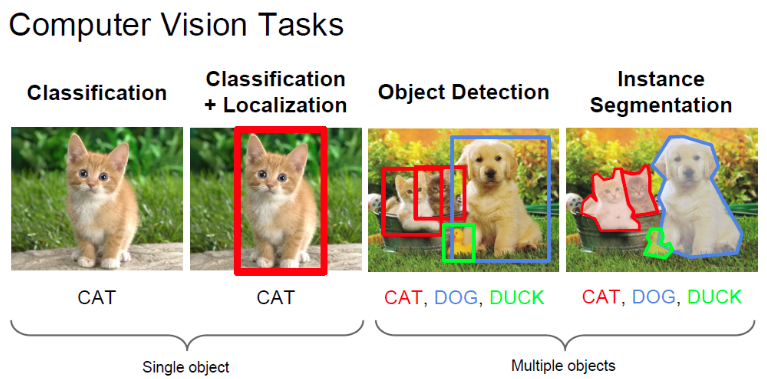
\includegraphics[width=0.8\textwidth]{img/computerVision.png}
    \caption{Tareas de Visión por computadora \cite{taskcompvision}}
    \label{fig:computer vision}
\end{figure}

\newpage
Este proyecto, optó por la \textit{Detección de objetos (Object Detection)} como herramienta principal para resolver la problemática de la identificación y localización de pivotes de riego y silobolsas en imágenes satélites, dada la naturaleza del problema: Hacer un conteo de la cantidad de estos objetos que se pueden encontrar en una determinada área de suelo.

\subsubsection{Conceptos}
Sin importar el modelo de Machine Learning subyacente, existen algunos conceptos dentro de lo que es Object Detection que son comunes a ésta aplicación y que ameritan ser explicados. Sin embargo, dado que el modelo seleccionado en este trabajo está basado en YOLO (You Only Look Once) \cite{yolo}, los conceptos a continuación se explican desde el punto de vista en el que son utilizados por YOLO.

\paragraph{Bounding box}
Cuando se realiza una predicción, el modelo ubica etiquetas (bounding box) en forma de recuadros sobre el objeto \cite{cnncourse}.

\begin{figure}[h!]
    \centering
    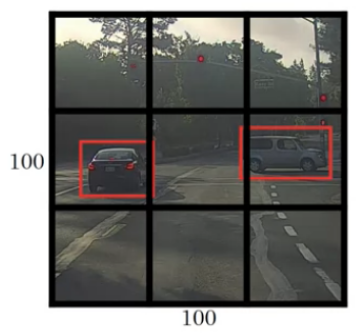
\includegraphics[width=0.6\textwidth]{img/bounding-box-yolo.png}
    \caption{Bounding Box in YOLO}
    \label{fig:bb in YOLO}
\end{figure}

YOLO divide la imagen en celdas, donde cada una de ellas se “encarga” de detectar los objetos cuyo centro de Bounding Box (BB) caiga dentro de ella. Figura \ref{fig:bb in YOLO} .

Cada celda arroja una salida con su predicción.
Dicha salida es un vector formado por: \[Y=\{Pc, Bx, By, Bh. Bw, C1, C2, C3\}\] con:
\begin{itemize}
    \item \textit{Pc = 0 o 1}: probabilidad de que haya un objeto en esa celda.
    \item \textit{Bx, By, Bh, Bw}: coordenadas (x, y, altura, ancho) para especificar el cuadro rojo delimitador del objeto asociado a esa celda.
    \item \textit{C1, C2, C3, …, Cn}: Probabilidades de las clases de objetos, por ejemplo puede ser las clases de peatón, coches y motocicletas.
\end{itemize}

\paragraph{Non-max suppression}
Es un algoritmo utilizado para que el modelo no detecte 2 veces el mismo objeto. Esto se debe a que YOLO realiza muchas predicciones sobre el mismo objeto, y de esta manera se realiza un filtrado seleccionando solo la mejor (Figura \ref{fig:non max supression}).
\\
\begin{figure}[h]
    \centering
    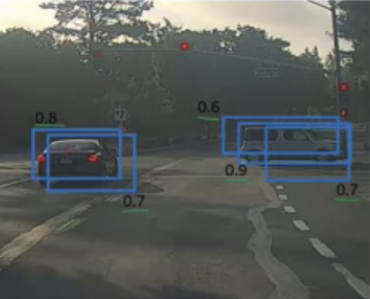
\includegraphics[width=0.6\textwidth]{img/non-max-supression-yolo.png}
    \caption{Non Max Supression in YOLO}
    \label{fig:non max supression}
\end{figure}

Procedimiento Non-max supression \cite{cnncourse} :
\begin{enumerate}
    \item Examina las probabilidades asociadas con cada una de las detecciones. 
    \item Selecciona el BB con el Pc más alto y lo elige como predicción parcial. Se descartan todos los BB con una \textit{Pc \leq 0.6}.

Si hay BB restantes:
    \item Descarta los BB remanentes con 0.5 o más de IoU contra el BB seleccionado en el punto anterior.
\end{enumerate}
Para el caso que haya varias clases, hay que correr Non-max una vez por cada clase, chequeando solamente los BB cuya predicción de clase sea la que se está chequeando en ese momento.

\newpage
\paragraph{Anchor Boxes}
Si dos o más objetos tienen el centro de su Bounding Box en la misma celda, el detector de objetos puede llegar a confundirse. Solución: Se pre-definen dos o más formas diferentes de cajas de anclaje o anchor boxes y se asocian tantas predicciones como anchor boxes haya. El anchor box que sea más similar a la forma del Bounding Box del objeto, será el asignado en el vector de salida \cite{cnncourse} (Figura \ref{fig:anchor boxes en YOLO}).

La elección de los tamaños y formas de los anchor boxes se puede elegir a mano, o tal vez 5 o 10 formas de anchor box, con una variedad suficiente como para cubrir todos los tipos de objetos que se quiere detectar.
También existe la posibilidad de realizar una selección más avanzada, es decir, automatizando la decisión, utilizando un algoritmo de machine learning llamado K-Means.
% \subsubsection{K-means}

\begin{figure}[p]
    \centering
    \begin{subfigure}[h!]{.5\textwidth}
        \centering
        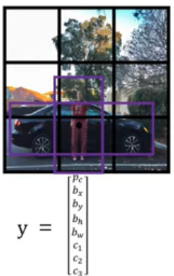
\includegraphics[width=\linewidth]{img/anchor-boxes-yolo-1.png}
        \caption{Output vector en YOLO}
    \end{subfigure}
    \begin{subfigure}[h!]{.6\textwidth}
        \raggedleft
        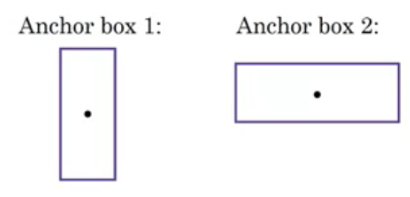
\includegraphics[width=\linewidth]{img/anchor-boxes-yolo-2.png}
        \caption{Ejemplos de Anchor Boxes en YOLO}
    \end{subfigure}
    \begin{subfigure}[h!]{.15\textwidth}
        \raggedright
        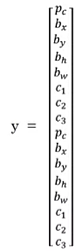
\includegraphics[width=\linewidth]{img/anchor-boxes-yolo-3.png}
        \caption{Output vector con 2 anchor boxes en YOLO}
    \end{subfigure}
    \caption{Anchor Boxes en YOLO}
    \label{fig:anchor boxes en YOLO}
\end{figure}

\newpage
\paragraph{Intersection Over Union}
La intersección sobre la Unión o Intersection over Union (IoU) \cite{iou}, es una  métrica de evaluación utilizada para medir la precisión de un detector de objetos en un conjunto de datos en particular. Sin embargo, hay que tener  en cuenta que el algoritmo real utilizado para generar las predicciones no importa. Cualquier algoritmo que proporcione cuadros delimitadores predichos como salida, puede evaluar su rendimiento usando IoU; como por ejemplo, YOLO. Para aplicar IoU (Figura \ref{fig:iou 1}) y evaluar un detector de objetos (arbitrario), necesitamos:

\begin{itemize}
    \item Ground-truth bounding box (es decir, los cuadros delimitadores etiquetados ``a mano'' del conjunto de prueba que especifican en qué parte de la imagen está nuestro objeto).
    \item Predicted bounding box, cuadros delimitadores predichos de el modelo.
\end{itemize}

\begin{figure}[h!]
    \centering
    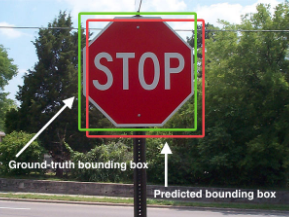
\includegraphics[width=0.6\textwidth]{img/iou-1.png}
    \caption{Ground Thruth and Predicted Bounding Box}
    \label{fig:iou 1}
\end{figure}

El objetivo, es calcular la intersección sobre la unión entre estos cuadros delimitadores. Ésta intersección se puede determinar a través de la siguiente fórmula:  Figura \ref{fig:iou formula}:

\begin{figure}[h!]
    \centering
    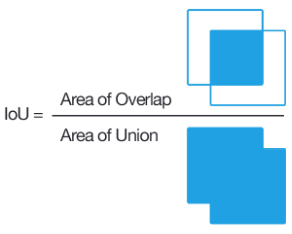
\includegraphics[width=0.5\textwidth]{img/iou-2.png}
    \caption{Intersetion over Union formula}
    \label{fig:iou formula}
\end{figure}

\newpage
\begin{itemize}
    \item En el numerador se calcula el  área de superposición entre el cuadro delimitador predicho y el cuadro delimitador de Ground-truth.
    \item El denominador es el  área de unión, o el área abarcada tanto por el cuadro delimitador predicho, como por el cuadro delimitador de Ground-truth.
\end{itemize}

Luego, dividir el área de superposición por el área de unión produce el puntaje final:  la Intersección Sobre la Unión - IoU. Una IoU mayor a 0.5 normalmente se considera una predicción ``buena''.

Cuando se entrena un detector de objetos, se necesita un conjunto de datos, que puede dividirse en dos grupos:

\begin{itemize}
    \item Un conjunto de entrenamiento utilizado para entrenar el detector de objetos.
    \item Un conjunto de pruebas para evaluar el detector de objetos.
\end{itemize}

Ambos conjuntos consistirán en:

\begin{itemize}
    \item Las imágenes en sí mismas.
    \item Los  cuadros delimitadores asociados con los objetos en la imagen, es decir, las coordenadas (x, y) del objeto en la imagen.
\end{itemize}

Estos cuadros delimitadores, para ambos conjuntos, están ``etiquetados a mano'' y, por lo tanto, son llamados ``ground-truth''. Su objetivo es tomar las imágenes de entrenamiento + cuadros delimitadores, construir un detector de objetos y luego evaluar su rendimiento en el conjunto de pruebas.

En la realidad, es  extremadamente  improbable que las  coordenadas (x, y) del Predicted bounding box coincidan exactamente con las coordenadas (x, y) del Ground-truth bounding box debido a los parámetros variables del modelo (como tamaño de ventana deslizante, método de extracción de características, etc.). Por ello, se necesita definir una métrica de evaluación que recompense los Predicted bounding box (rojo) por superponerse en gran medida con el Ground-truth (verde). 

\begin{figure}[h!]
    \centering
    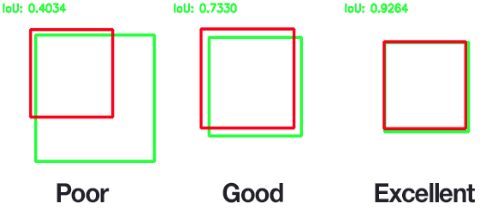
\includegraphics[width=0.6\textwidth]{img/iou-3.png}
    \caption{Intersetion over Union examples}
    \label{fig:iou ejemplos}
\end{figure}

Como se puede ver en la imagen \ref{fig:iou ejemplos}, los Predicted bounding box que se superponen en gran medida con los Ground-truth bounding box tienen puntajes más altos que aquellos con menos superposición. Esto hace que Intersection over Union sea una métrica excelente para evaluar detectores de objetos personalizados.


\newpage